%%%%%%%%%%%%%%%%%%%%%%%%%%%%%%%%%%%%%%%%%%%%%%%%%%%%%%%%%%%%%%%%%%%%%%%%%%%%%%%%
% ISE Lab -- Topic
% Giovanni Ciatto
% Alma Mater Studiorum - Università di Bologna
% mailto:giovanni.ciatto@unibo.it
%%%%%%%%%%%%%%%%%%%%%%%%%%%%%%%%%%%%%%%%%%%%%%%%%%%%%%%%%%%%%%%%%%%%%%%%%%%%%%%%
%\documentclass[handout]{beamer}\mode<handout>{\usetheme{default}}
%
\documentclass[presentation]{beamer}\mode<presentation>{\usetheme{AMSBolognaFC}}
%\documentclass[handout]{beamer}\mode<handout>{\usetheme{AMSBolognaFC}}
%%%%%%%%%%%%%%%%%%%%%%%%%%%%%%%%%%%%%%%%%%%%%%%%%%%%%%%%%%%%%%%%%%%%%%%%%%%%%%%%
\usepackage{ise-lab-common}
\usepackage{psyki-tutorial}
%%%%%%%%%%%%%%%%%%%%%%%%%%%%%%%%%%%%%%%%%%%%%%%%%%%%%%%%%%%%%%%%%%%%%%%%%%%%%%%%
\title[SKI via \psyki{}]{Symbolic Knowledge Injection via \psyki{}}
%
\subtitle{A tutorial}
%
\author[\sspeaker{\gcShort} et al.]{
    \speaker{\gcFull} \and Matteo Magnini
    \\
    \gcEmail \and \ttemail{matteo.magnini@unibo.it}
}
%
\institute[\uniboShort]{
    \disi{} (\disiShort)\\\unibo, Cesena, Italy
}
%
\date[PRIMA 2022]{
    $24^{th}$ International Conference on 
    \\
    Principles and Practice of Multi-Agent Systems
    \\
    November 16, 2022
}
%
%%%%%%%%%%%%%%%%%%%%%%%%%%%%%%%%%%%%%%%%%%%%%%%%%%%%%%%%%%%%%%%%%%%%%%%%%%%%%%%%
\begin{document}
%%%%%%%%%%%%%%%%%%%%%%%%%%%%%%%%%%%%%%%%%%%%%%%%%%%%%%%%%%%%%%%%%%%%%%%%%%%%%%%%

%/////////
\frame{\titlepage}
%/////////

%%===============================================================================
\section*{Outline}
%%===============================================================================
%
%%/////////
\frame[c]{\tableofcontents[hideallsubsections]}
%%/////////

%===============================================================================
\section{What and Why}
%===============================================================================

\begin{frame}%[allowframebreaks]
    \frametitle{What}

    \alert{\psyki}: a (Python) platform for symbolic knowledge injection

    \begin{columns}
        \begin{column}{.3\linewidth}
            \centering
            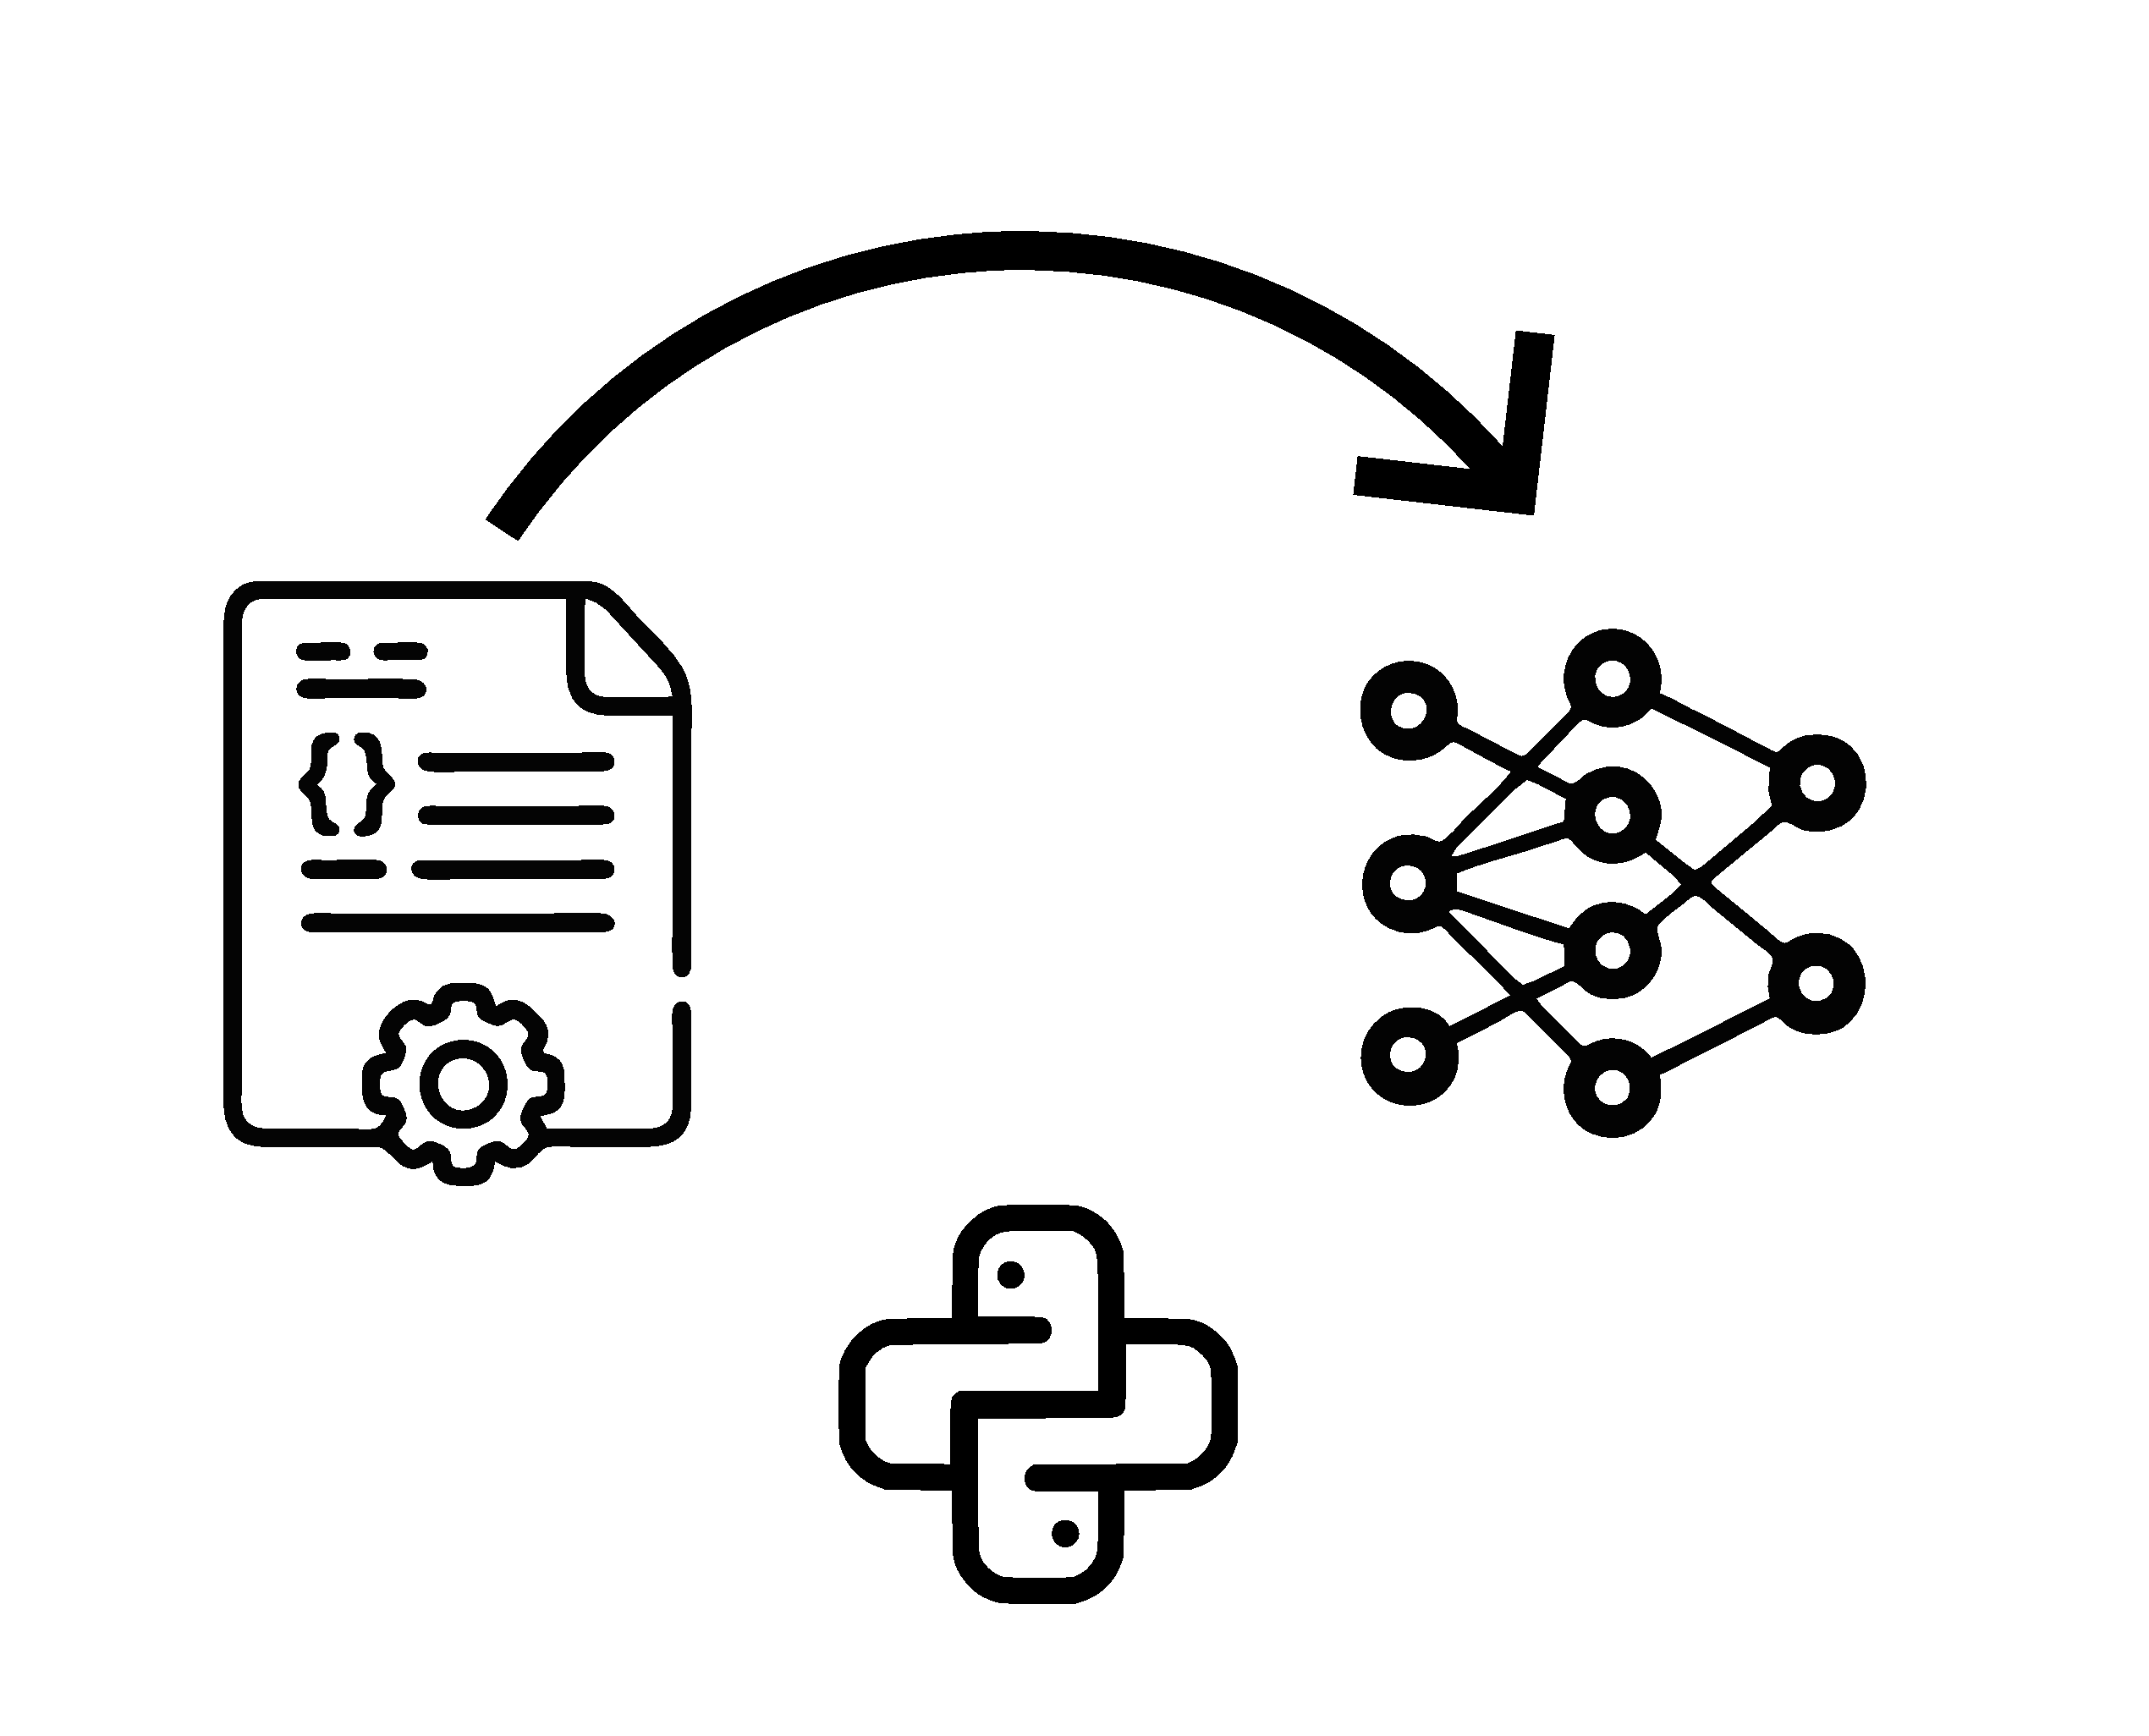
\includegraphics[width=\linewidth]{./figures/psyki-logo.pdf}
        \end{column}
        \begin{column}{.7\linewidth}
            \begin{block}{GitHub Repository}\centering
                \alert{\url{https://github.com/psykei/psyki-python}}

                \tiny{(please star us :)}
            \end{block}

            \begin{block}{Main papers}
                \begin{itemize}
                    \item \cite{psyki-extraamas2022}
                \end{itemize}
            \end{block}
        \end{column}
    \end{columns}
\end{frame}

% \begin{frame}[c]{Why}
%     \begin{itemize}
%         \item Pervasive adoption of \alert{sub-symbolic}, ML-based predictors in AI
        
%         \vfill

%         \item Their \alert{opacity}\ccite{Lipton2018} brings \alert{drawbacks}\ccite{guidotti2018survey}:
%         %
%         \vfill
%         %
%         \begin{itemize}\small
%             \item difficulty in \alert{spotting} unintendedly learnt knowledge
            
%             \vfill
            
%             \item difficulty in spotting ``\alert{bugs}'' in what a numeric predictor has learnt
            
%             \vfill
            
%             \item difficult to learn upon \alert{lacking data} 
                        
%             \vfill
            
%             \item difficult to transfer \alert{human's common-sense} to sub-symbolic AI
            
%         \end{itemize}

%         \vfill

%         \item[$\rightarrow$] Need to \alert{make} ML predictors \alert{predictable}
%         %
%         \begin{itemize}
%             \item by finely \alert{controlling} what that learn
%         \end{itemize}
%     \end{itemize}
% \end{frame}

%/////////
\begin{frame}[c]{Why SKI?}
    %
    There are several benefits:
    %
    \begin{itemize}
        %
        \item prevent the predictor to become a black-box\alert{!};
        %
        \item reduce learning time;
        %
        \item reduce the data size needed for training;
        %
        \item improve predictor's accuracy;
        %
        \item build a predictor that behave as a logic engine.
    \end{itemize}
    %
\end{frame}
%/////////

%===============================================================================
\section{Background}
%===============================================================================

\begin{frame}[allowframebreaks]{Symbolic Knowledge Injection}
    Key insights:
    %
    \medskip
    %
    \begin{itemize}
        \item \alert{Altering} ML predictors\ldots
        \medskip
        \item \ldots to make they \alert{comply} to user-provided knowledge\ldots
        \medskip
        \item \ldots which is represented in \alert{symbolic form}
    \end{itemize}

    \framebreak

    \begin{block}{We define SKI as:}
        any \alert{algorithmic} procedure affecting how \alert{sub-symbolic predictors} draw their inferences in such a way that predictions are either \alert{computed} as a function of, or made \alert{consistent} with, some \alert{given} \alert{symbolic knowledge}*.
    \end{block}
    %
    \bigskip
    %
    * a wide definition that includes the vast majority of the works surveyed in \cite{surveyNeuroSymb,surveyXie,surveyCalegariCO20}.

    \framebreak

    General workflow:
    %
    \begin{figure}
        \centering
        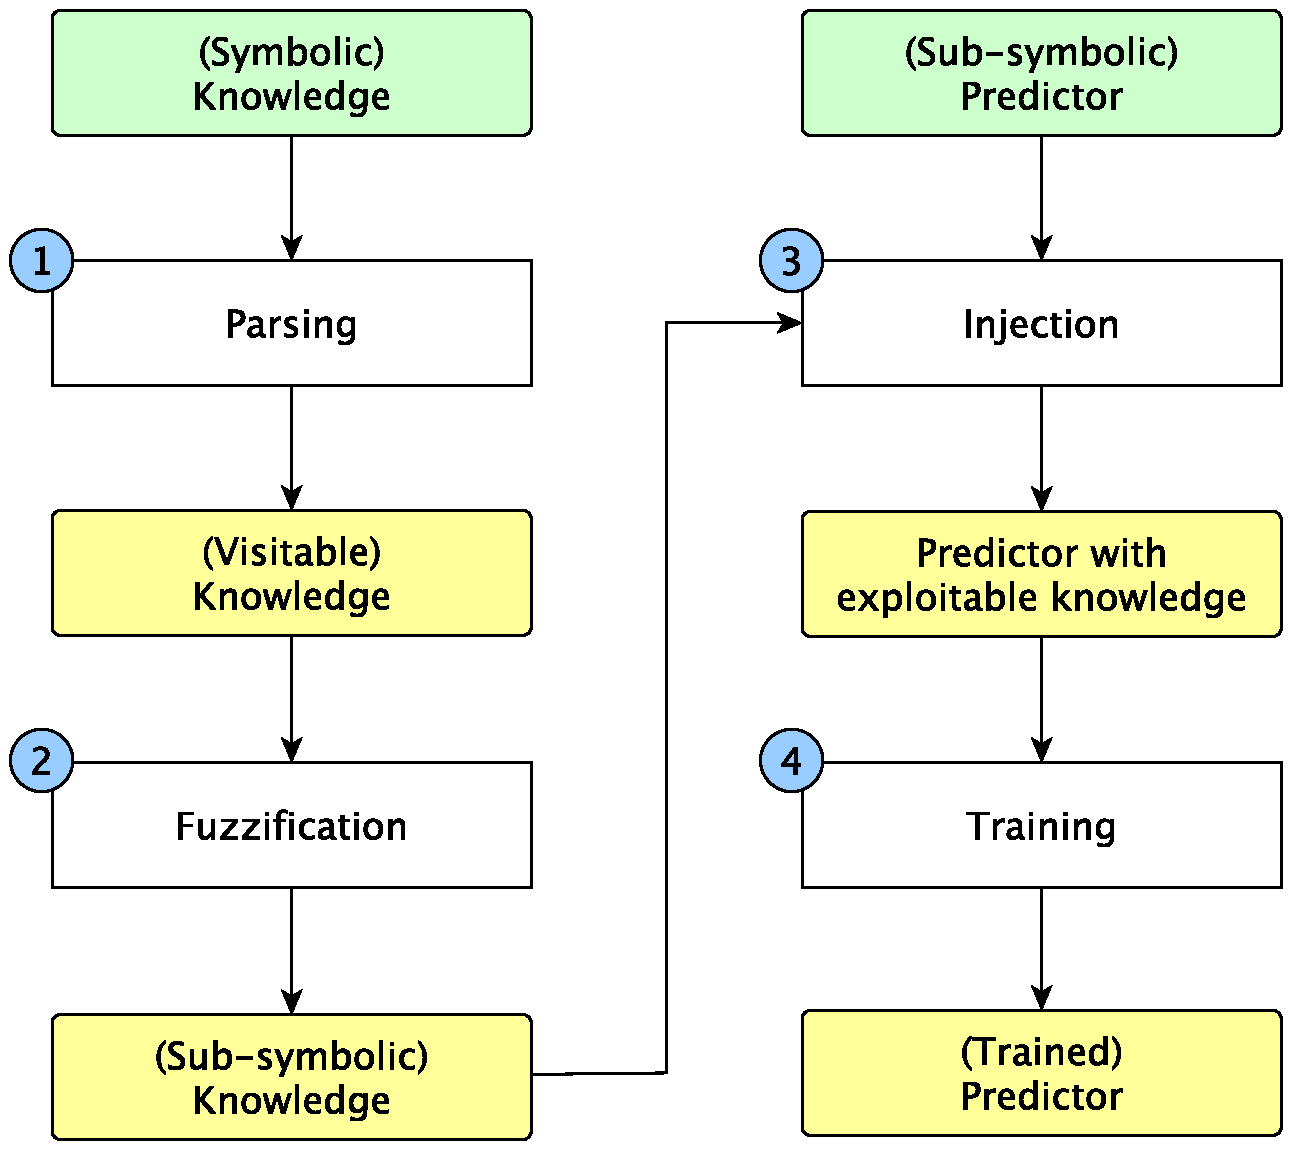
\includegraphics[width=0.8\textheight]{figures/ski-workflow.pdf}
    \end{figure}
\end{frame}

\begin{frame}[allowframebreaks]{What does `symbolic' actually mean?}
    According to \cite{Gelder90}, \alert{symbolic} representations of knowledge
    %
    \begin{itemize}
        \item involves a \alert{set of symbols},
        \item which can be combined (e.g., concatenated) in (possibly) \alert{infinitely many} ways, 
        \item following precise \alert{syntactical} rules, and
        \item where both elementary symbols and any admissible combination of them can be assigned with \alert{meaning}
        %
        \begin{itemize}
            \item[ie] \alert{each} symbol can be mapped into some entity from the domain at hand.
        \end{itemize}
    \end{itemize}
    
    \begin{exampleblock}{Notable example}
        \begin{itemize}
            \item formal logic
        \end{itemize}
    \end{exampleblock}

    \framebreak

    \begin{alertblock}{Opposite notion: \textbf{distributed} representations}
        \begin{itemize}
            \item where symbols \alert{alone} have no meaning
            \item unless it is considered along with its \alert{neighbourhood}
            %
            \begin{itemize}
                \item[ie] any other symbol which is \alert{close} (according to some notion of closeness)
            \end{itemize}
        \end{itemize}
    \end{alertblock}
\end{frame}

% \begin{frame}[allowframebreaks]{Plenty of SKI methods from the literature}
%     \input{tables/ski.tex}
% \end{frame}

\begin{frame}[allowframebreaks]{Taxonomy of SKI methods}
    \begin{center}
        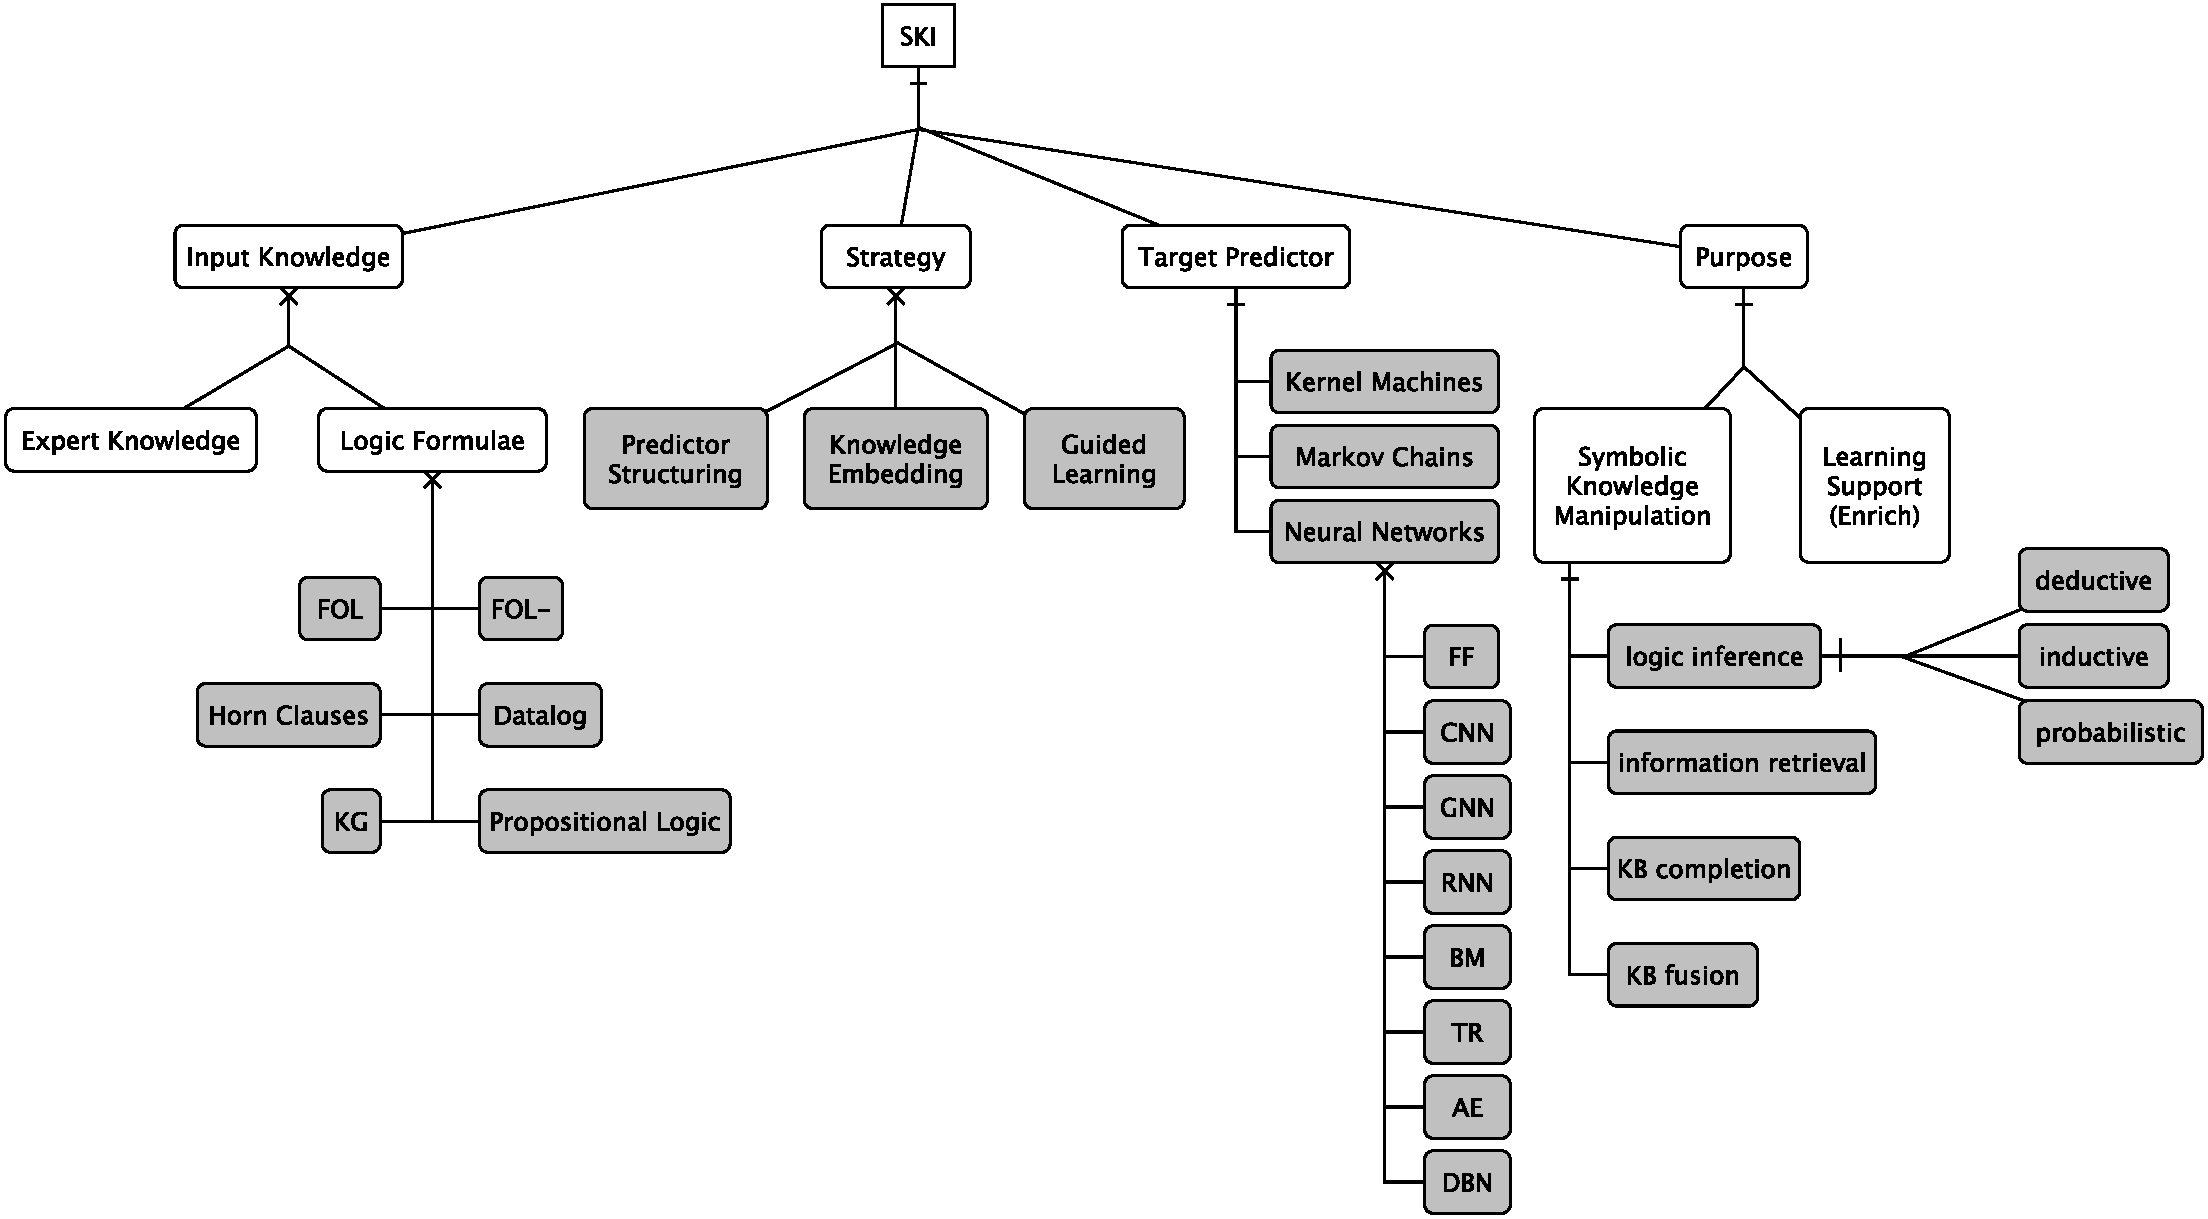
\includegraphics[width=\linewidth]{figures/ski-taxonomy.pdf}
    \end{center}
    
    \framebreak

    \begin{itemize}
        \item \alert{input knowledge} how is the knowledge to-be-injected represented?
        %
        \begin{itemize}
            \item commonly, some sub-set of first-order logic (FOL)
        \end{itemize} 

        \item \alert{target predictor} which predictors can knowledge be injected into?
        %
        \begin{itemize}
            \item mostly, neural networks
        \end{itemize} 

        \item \alert{strategy} how does injection actually work?
        %
        \begin{itemize}
            \item \alert{guided learning} the input knowledge is used to \alert{guide the training} process
            \item \alert{structuring} the \alert{internal} composition of the predictor is \alert{(re-)structured} to reflect the input knowledge  
            \item \alert{embedding} the input knowledge is \alert{converted} into numeric array form
        \end{itemize} 

        \item \alert{purpose} why is knowledge injected in the first place?
        %
        \begin{itemize}
            \item \alert{knowledge manipulation} improve / extend / reason about symbol knowledge---subsymbolically
            \item \alert{learning support} improve the sub-symbolic predictor (e.g. speed, size, etc.)
        \end{itemize} 

    \end{itemize}
\end{frame}

\subsection{Focus on input knowledge}

%/////////
\begin{frame}[allowframebreaks]{About Logic}

    How to represent knowledge?
    %
    \begin{center}
        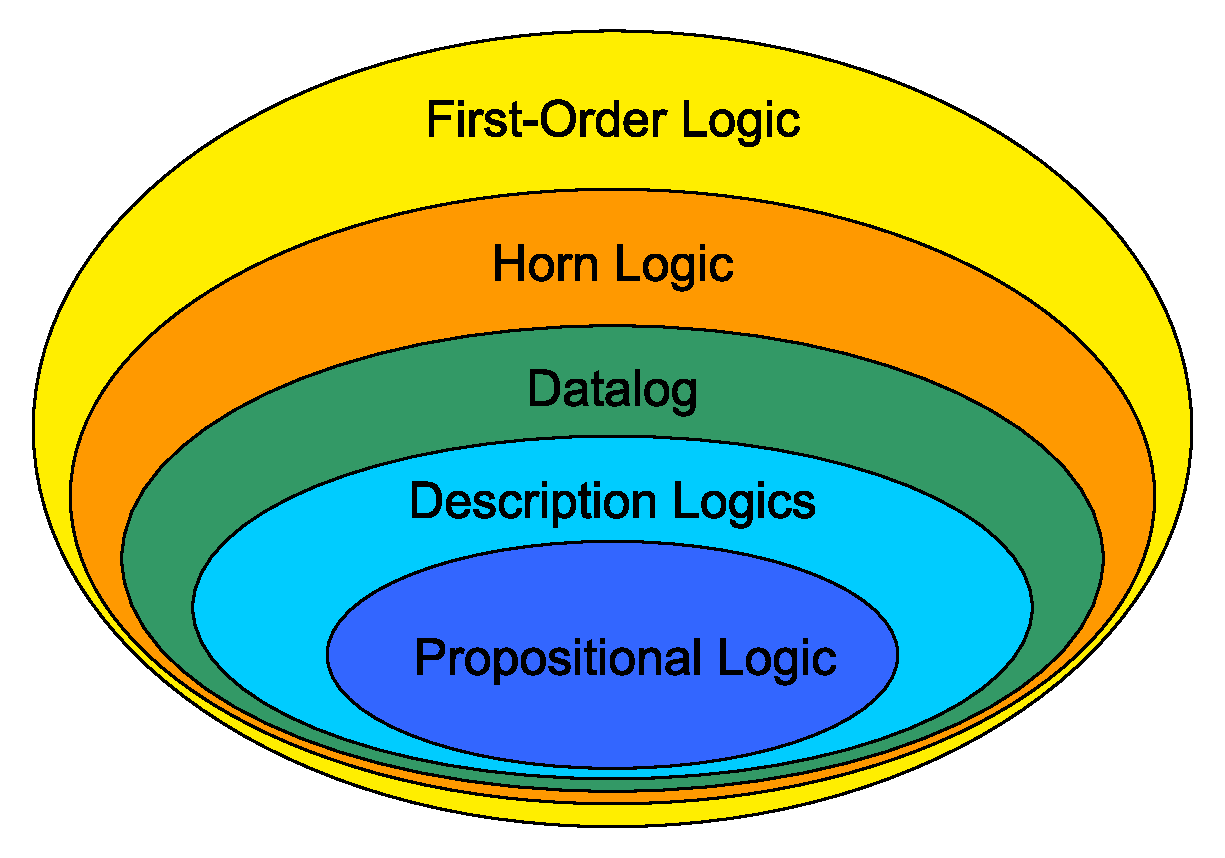
\includegraphics[width=.5\linewidth]{figures/venn-logic-diagram.pdf}
    \end{center}
    %
    \begin{itemize}
        \item \emph{expressiveness--tractability} trade-off\ccite{LevesqueB87, BrachmanL2004}
    \end{itemize}

    % \begin{block}{Intensional}
    %     \begin{itemize}
    %         \item indirect representation of data,
    %         %
    %         \item define a relation/set by describing its elements via other relations/sets.
    %     \end{itemize}
    %     %
    % \end{block}
    % %
    % \begin{block}{Extensional}
    %     \begin{itemize}
    %         \item direct representation of data,
    %         %
    %         \item explicit definition of entities involved.
    %     \end{itemize}
    % \end{block}
    % %
    % Recursive intensional predicates are very expressive and powerful, as they enable the description of infinite sets via a finite (and commonly small) amount of formul\ae.
    
    \framebreak        
    
    In practice, virtually all SKI algorithms deal with:
    %
    \begin{itemize}
        \item \alert{datalog};
        %
        \item description logics (a.k.a. \alert{knowledge graph}, KG);
        %
        \item \alert{propositional logic} (PL).
    \end{itemize}
\end{frame}
%/////////
    
%/////////
\begin{frame}[allowframebreaks]{First Order Logic}
    \begin{block}{Overview}
        \begin{itemize}
            \item FOL is extremely flexible and expressive
            %
            \begin{itemize}
                \item variables, quantifiers, structured terms, negation, logic connectives
            \end{itemize}
            
            \bigskip
    
            \item one can use \alert{recursion} to define recursive structures;
            %
            \begin{itemize}
                \item possibly, \alert{intensionally}---i.e. without \alert{extensively} describing everything
            \end{itemize}
    
            \bigskip
    
            \item maybe too ``powerful'' for canonical NN
            \begin{itemize}
                \item most NN are essentially DAG
                \item training via backpropagation\ccite{backpropagation} requires no cycles
                \item[$\rightarrow$] recursion not supported
            \end{itemize}
        \end{itemize}
    \end{block}

    \framebreak
    
    \begin{exampleblock}{Example of FOL knowledge base (Peano numbers)}
        \begin{equation*}
            \begin{array}{l}
                \pred{natural}(\const{zero})
                \\
                \forall\var{X} : \pred{natural}(\var{X}) \rightarrow \pred{natural}(\const{successorOf}(var{X})) 
            \end{array}    
        \end{equation*}
    \end{exampleblock}
\end{frame}
%/////////

%/////////
\begin{frame}[allowframebreaks]{Horn Clauses ($\approx$ Prolog)}
    \begin{block}{Overview}
        \begin{itemize}
            \item sub-set of FOL with:
            %
            \begin{itemize}
                \item implicit quantifiers
                \item limited set of logic connectives
            \end{itemize}
    
            \bigskip
    
            \item still supports recursion
    
            \bigskip
    
            \item nice expressiveness--tractability trade-off
            %
            \begin{itemize}
                \item often exploited to design/realise automatic reasoning
            \end{itemize}
        \end{itemize}
    \end{block}

    \framebreak
    
    \begin{exampleblock}{Example of Horn clauses (Peano numbers)}
        \begin{equation*}
            \begin{array}{l}
                \pred{natural}(\const{zero})
                \\
                \pred{natural}(\const{successorOf}(var{X})) \leftarrow \pred{natural}(\var{X})
            \end{array}    
        \end{equation*}
    \end{exampleblock}
\end{frame}
%/////////

%/////////
\begin{frame}[allowframebreaks]{Datalog}
    \begin{block}{Overview}
        \begin{itemize}
            \item sub-set of Horn clauses with \alert{no recursion}
    
            \bigskip
    
            \item good for SKI!
        \end{itemize}
    \end{block}
    
    \begin{exampleblock}{Peano numbers in Datalog}
        \begin{itemize}
            \item cannot be represented!
            %
            \begin{itemize}
                \item (as they require recursion)
            \end{itemize}
        \end{itemize}
    \end{exampleblock}
\end{frame}
%/////////

%/////////
\begin{frame}[allowframebreaks]{Description Logics ($\approx$ Knowledge Graphs)}
    
    \begin{block}{Overview}
        \begin{itemize}
            \item Very restricted subset of FOL
            %
            \begin{itemize}
                \item only constants, variables and $n$-ary predicates with $n \leq 2$;
            \end{itemize}

            \medskip
    
            \item Everything is represented via \alert{collections of triplets} of the form:
            \[\langle \functor{a}\ \predication{f}\ \functor{b} \rangle \text{ or } \predication{f}(\functor{a}, \functor{b})\]
            %
            where $\functor{a}, \functor{b}$ are \alert{entities}, and $\predication{f}$ is a (binary) \alert{relationship}

            \medskip
            
            \item essentially, directed graph:
            %
            \begin{itemize}
                \item nodes (i.e. entities) represent \alert{individuals},
                \item edges (i.e. relationships) represent \alert{relations} among individuals;
            \end{itemize}
        \end{itemize}
    \end{block}
    
    \framebreak
    
    \begin{figure}
        \centering
        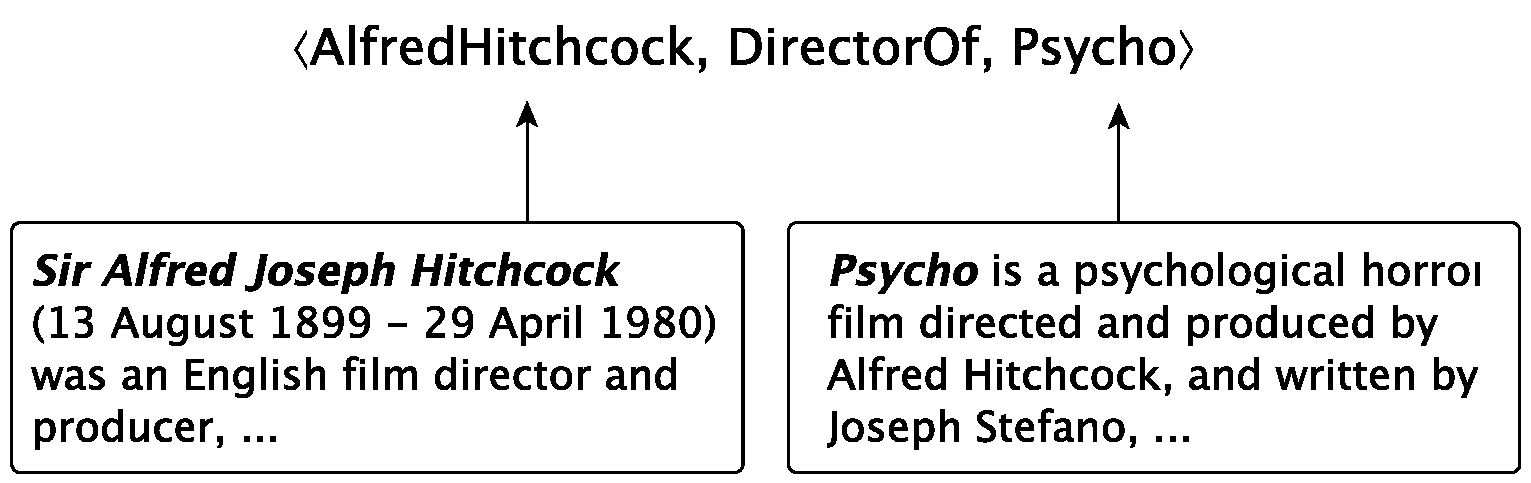
\includegraphics[width=0.8\textwidth]{figures/kg-example}
    \end{figure}    
\end{frame}    
%/////////
    
%/////////
\begin{frame}[allowframebreaks]{Propositional Logic}
    \begin{block}{Overview}
        \begin{itemize}
            \item The simplest subset of FOL
            %
            \begin{itemize}
                \item no quantifiers, no terms, no $n$-ary predicates with $n>0$
                \item essentially, just Boolean algebra 
            \end{itemize}

            \bigskip

            \item low expressiveness, but easy to work with.
        \end{itemize}
    \end{block}
    
    \begin{exampleblock}{Example}
        \begin{equation*}
            \begin{aligned}
                \pred{big\_petal}\wedge\pred{average\_sepal}&\rightarrow\const{virginica}.\\
                \pred{big\_petal}\wedge\neg\pred{average\_sepal}&\rightarrow\const{versicolor}.\\
                \pred{big\_petal}&\rightarrow\const{setosa}.\\
                \pred{average\_sepal}&\equiv(3\le\var{SepalWidth}<5)\\
                \pred{big\_petal}&\equiv(\var{PetalLength}>3)\\
            \end{aligned}    
        \end{equation*}
    \end{exampleblock}
\end{frame}
%/////////

\subsection{Focus on strategy}

%/////////
\begin{frame}[allowframebreaks]{Strategy 1: Guided Learning}

    \begin{figure}
        \centering
        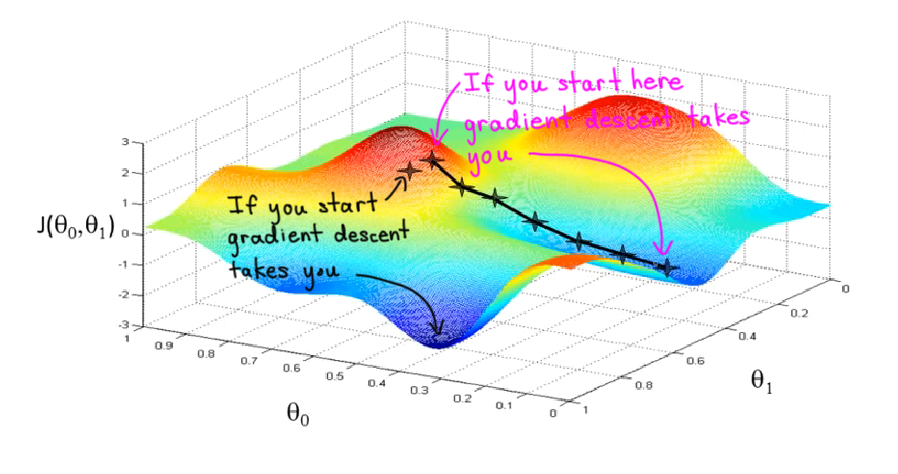
\includegraphics[width=0.7\linewidth]{figures/nn-gradient-descent.png}
    \end{figure}   
    %
    \begin{itemize}
        \item learning is essentially an \alert{optimizionation} process
        \item \ldots often performed via \alert{gradient descent}
        %
        \begin{itemize}
            \item[ie] minimising a \alert{loss function}
        \end{itemize}
    \end{itemize}

    \framebreak

    \begin{block}{SKI via Guided Learning}
        \begin{enumerate}
            \item Input knowledge is converted into a \alert{cost factor} 
            %
            \begin{itemize}
                \item[ie] the more the knowledge is violated, the higher the cost
            \end{itemize}
            
            \item The loss function is altered to \alert{include} that cost factor
            %
            \begin{itemize}
                \item[eg] as a simple additive regularisation factor
            \end{itemize}
            
            \item The predictor is then trained \alert{as usual}
            
            \medskip

            \item[$\rightarrow$] Training minimises both the predictors' \alert{error} and \alert{inconsistency} w.r.t. knowledge
        \end{enumerate}
    \end{block}
    %
    \begin{figure}
        \centering
        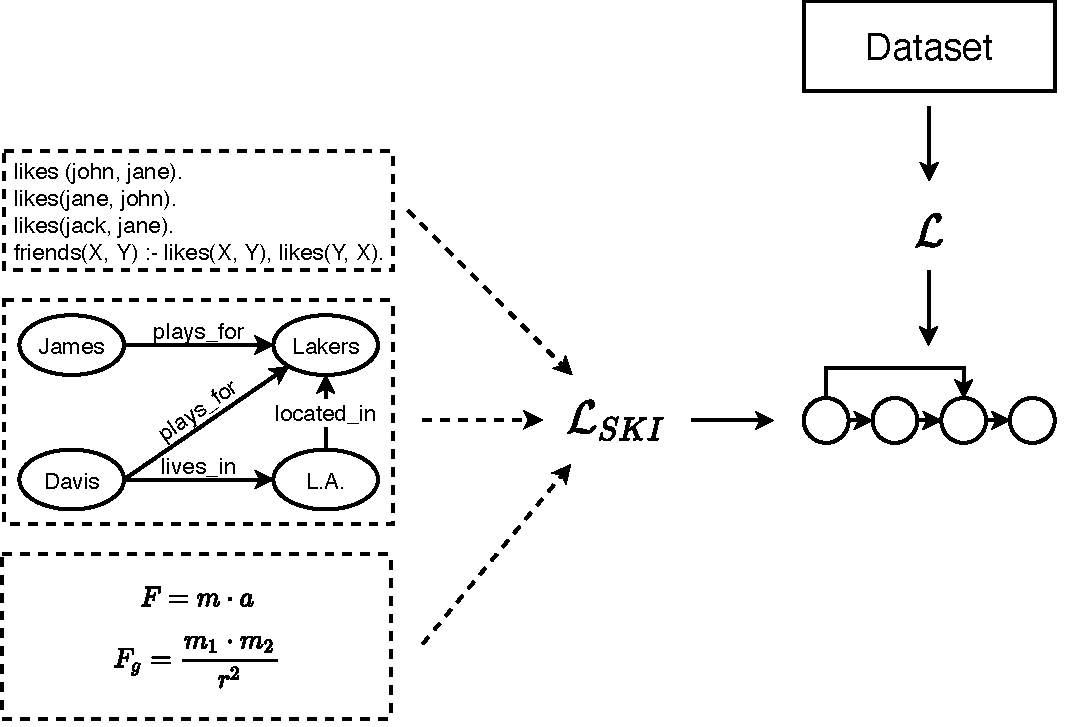
\includegraphics[width=0.6\textwidth]{figures/ski-constraining}
    \end{figure}
     
\end{frame}
%/////////

%/////////
\begin{frame}[allowframebreaks]{Strategy 2: Structuring}
    \begin{block}{SKI via Guided Learning}
        \begin{itemize}
            \item The predictor's inner architecture is shaped  to``mimic'' the knowledge
            
            \item Shaping is predictor-dependent
            %
            \begin{itemize}
                \item[eg] for neural networks, this means creating \alert{ad-hoc layers}
                %
                \begin{itemize}
                    \item where small groups of neurons are used to compute pieces of a formula
                \end{itemize}
            \end{itemize}

            \medskip
            
            \item[$\rightarrow$] The predictor directly exploits the knowledge during inference
        \end{itemize}
    \end{block}
    %
    \begin{figure}
        \centering
        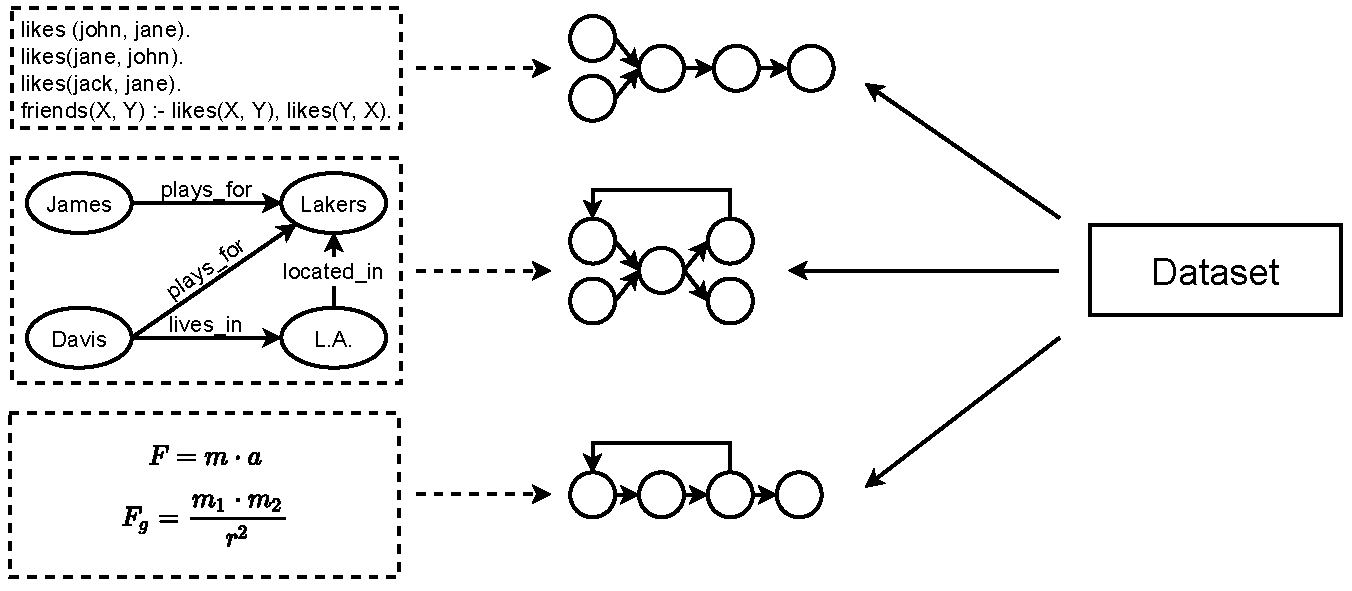
\includegraphics[width=0.7\textwidth]{figures/ski-structuring}
    \end{figure}

    \framebreak
    
    Example:
    %
    \begin{columns}
        \column{.48\linewidth}
        \begin{equation*}
            \begin{aligned}
                \var{A}&\leftarrow\var{B}\wedge\var{C}\wedge\neg\var{D}.\\
                \var{A}&\leftarrow\var{E}\wedge\var{F}.\\
                \var{B}&\leftarrow\const{true}.\\
            \end{aligned}    
        \end{equation*}
        \column{.04\linewidth}
        \centering $\leftrightarrow$
        \column{.48\linewidth}
        \begin{figure}
            \centering
            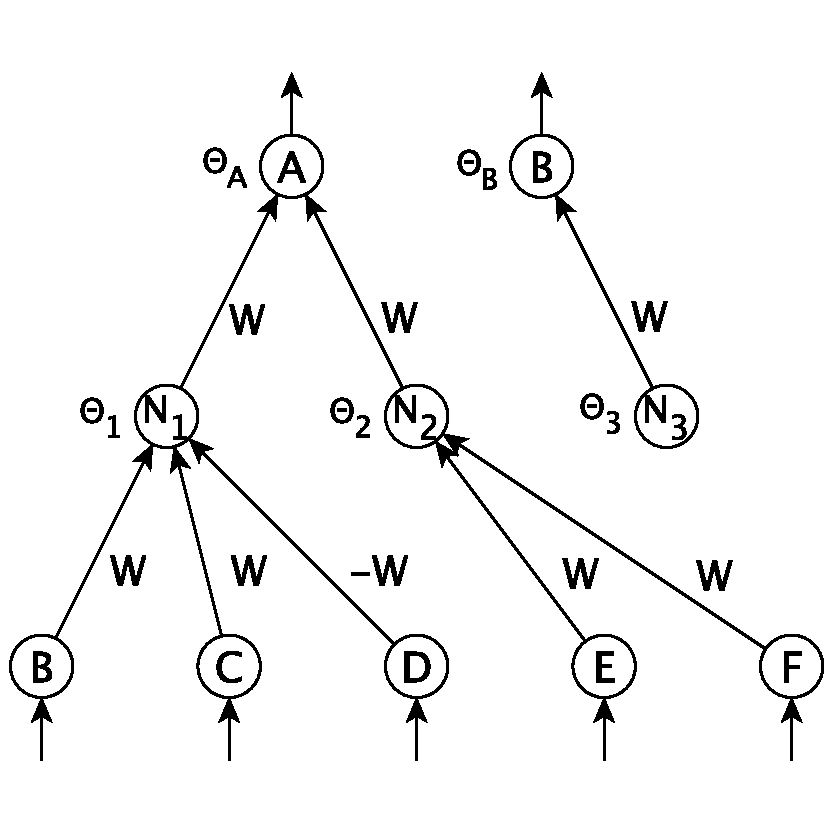
\includegraphics[width=\linewidth]{figures/structuring-example}
        \end{figure}
    \end{columns}
\end{frame}
%/////////

%/////////
\begin{frame}[allowframebreaks]{Strategy 3: Embedding}
    
    \begin{block}{SKI via Guided Learning}
        \begin{itemize}
            \item Input knowledge is converted into numeric tensor(s)
            %
            \item These are used as the training set for an ordinary learning process
            
            \medskip
            
            \item[$\rightarrow$] The predictor is trained and used `as usual'
        \end{itemize}
    \end{block}
    
    \begin{figure}
        \centering
        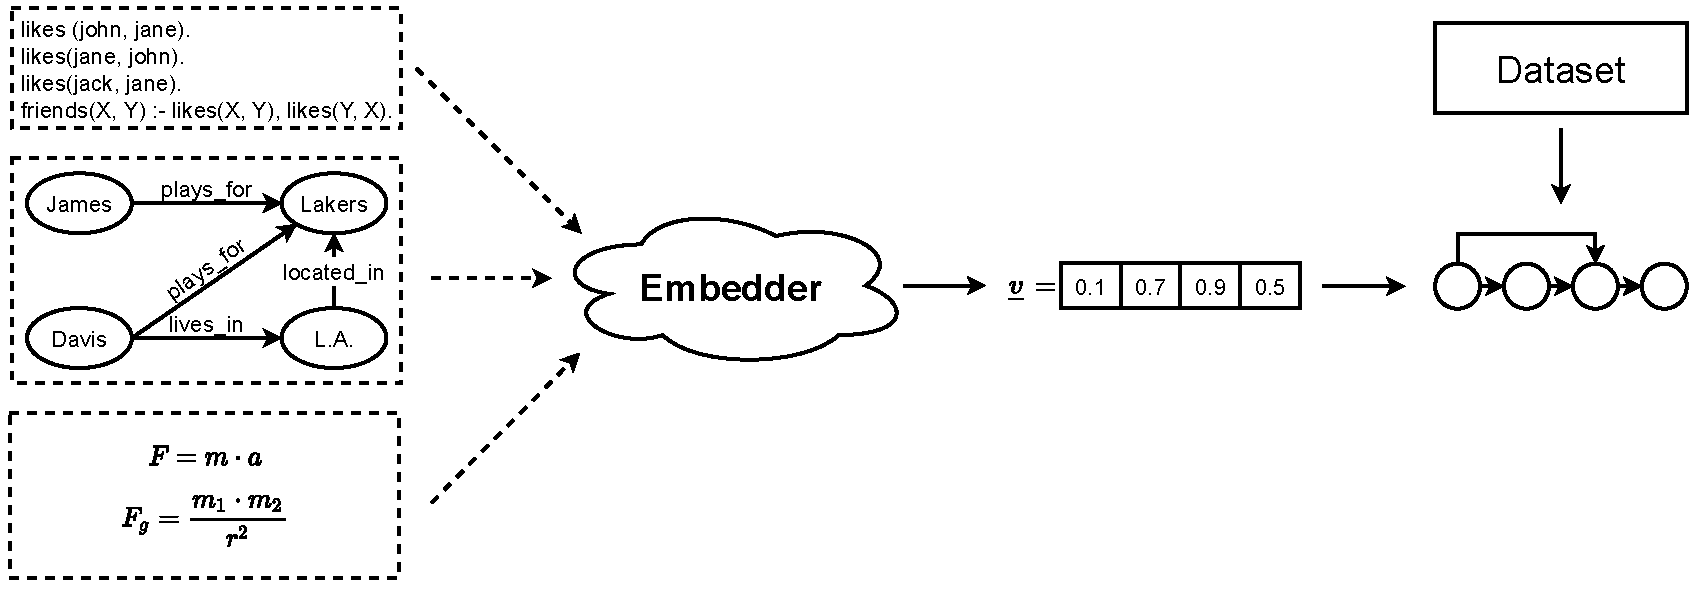
\includegraphics[width=0.7\textwidth]{figures/ski-embedding}
    \end{figure}
    
    \framebreak
    
    Example: \alert{knowledge graph embedding}\ccite{kge-survey}
    %
    \begin{itemize}
        \item \alert{entities} and \alert{relations} are embedded into continuos vector spaces;
        %
        \item scoring function $f_{r}(h,t)$ defined on each fact $(h, r, t)$ to measure its plausibility;
    \end{itemize}
    %
    \begin{figure}
        \centering
        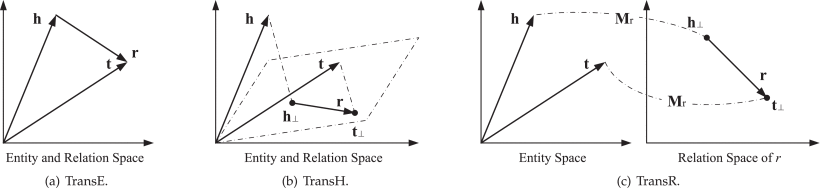
\includegraphics[width=0.8\textwidth]{figures/kge-space.png}
    \end{figure}

    \framebreak
    
    \begin{figure}
        \centering
        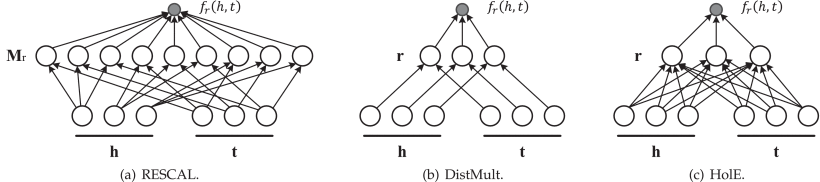
\includegraphics[width=0.8\textwidth]{figures/kge-nn-1.png}
    \end{figure}

    \begin{figure}
        \centering
        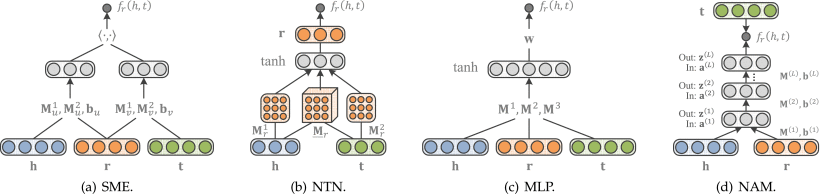
\includegraphics[width=0.8\textwidth]{figures/kge-nn-2.png}
    \end{figure}
    
\end{frame}
%/////////

\subsection{Example algorithms}

%/////////
\begin{frame}[allowframebreaks]{Knowledge Injection via Network Structuring\ccite{kins-cilc2022}}
    
    \begin{block}{KINS}
        %
        A general SKI algorithm that does not impose constrains on the sub-symbolic predictor to enrich.
        %
        \begin{description}
            %
            \item[purpose] $\rightarrow$ learning support;
            %
            \item[target predictor] $\rightarrow$ neural networks;
            %
            \item[strategy] $\rightarrow$ structuring;
            %
            \item[input logic] $\rightarrow$ stratified Datalog with negation.
            %    
        \end{description}        
    \end{block}

    \framebreak
    
    \begin{figure}
        \centering
        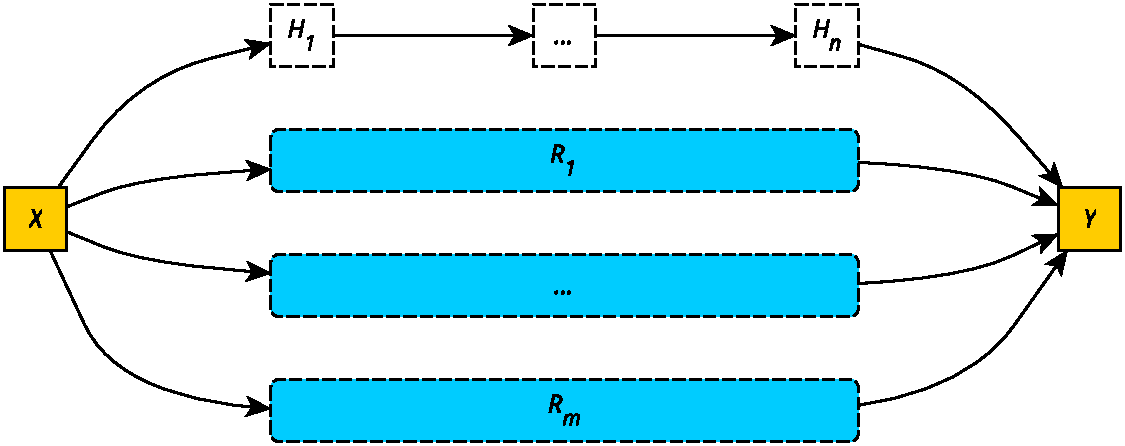
\includegraphics[width=0.8\textwidth]{figures/kins-architecture}
    \end{figure}

    \framebreak
    
    \resizebox{\textwidth}{!}{
    \begin{tabular}{l|r||l|r}
        \textbf{Formula} & \textbf{C. interpretation} & \textbf{Formula} & \textbf{C. interpretation}
        \\
        \hline\hline
        $\llbracket\neg \phi\rrbracket$ & $\eta(1 - \llbracket\phi\rrbracket)$ & $\llbracket\phi \le \psi\rrbracket$  & $\eta(1 + \llbracket \psi \rrbracket - \llbracket \phi \rrbracket)$  % Negation % Less equal
        \\
        $\llbracket\phi  \wedge \psi\rrbracket$ &  $\eta(min(\llbracket\phi\rrbracket, \llbracket\psi\rrbracket))$ &  $\llbracket \pred{class}(\bar{X}, \const{y}_i) \leftarrow \psi \rrbracket$ & $\llbracket \psi \rrbracket^{*}$ % Conjunction % Class
        \\
        $\llbracket\phi  \vee \psi\rrbracket$ & $\eta(max(\llbracket\phi\rrbracket, \llbracket\psi\rrbracket))$ & $\llbracket \text{expr}(\bar{X}) \rrbracket$ & $\text{expr}(\llbracket\bar{X}\rrbracket)$ % Disjunction
        \\
        $\llbracket\phi = \psi\rrbracket$ & $\eta(\llbracket\neg( \phi \ne \psi )\rrbracket )$ &$\llbracket \mathtt{true} \rrbracket$ & $1$ % Equal
        \\
        $\llbracket\phi \ne \psi\rrbracket$ & $\eta(|\llbracket\phi\rrbracket-\llbracket\psi\rrbracket|)$ & $\llbracket \mathtt{false} \rrbracket$ & $0$ % Not Equal
        \\
        $\llbracket\phi > \psi\rrbracket$ & $\eta(max(0, \frac{1}{2} + \llbracket\phi\rrbracket - \llbracket\psi\rrbracket))$ & $\llbracket X \rrbracket$ & $x$ % Greater
        \\
        $\llbracket\phi \ge \psi\rrbracket$  & $\eta(1 + \llbracket \phi \rrbracket - \llbracket \psi \rrbracket)$ & $\llbracket \const{k} \rrbracket$ & $k$ % Greater Equal
        \\
        $\llbracket\phi < \psi\rrbracket$  &  $\eta(max(0, \frac{1}{2} + \llbracket\psi\rrbracket - \llbracket\phi\rrbracket))$ & $\llbracket \pred{p}(\bar{X}) \rrbracket^{**}$ & $\llbracket \psi_1 \vee \ldots \vee \psi_k \rrbracket$ % Less 
      
    \end{tabular}
}
\begin{center}\scriptsize
    $^{*}$ encodes the value for the $i^{th}$ output
    \\
    \smallskip
    $^{**}$ assuming $p$ is defined by $k$ clauses of the form:
    \\
    $\pred{p}(\bar{X}) \leftarrow \psi_1,\ \ldots,\ \pred{p}(\bar{X}) \leftarrow \psi_k$
\end{center}
    
    \framebreak
    
    \begin{figure}
        \centering
        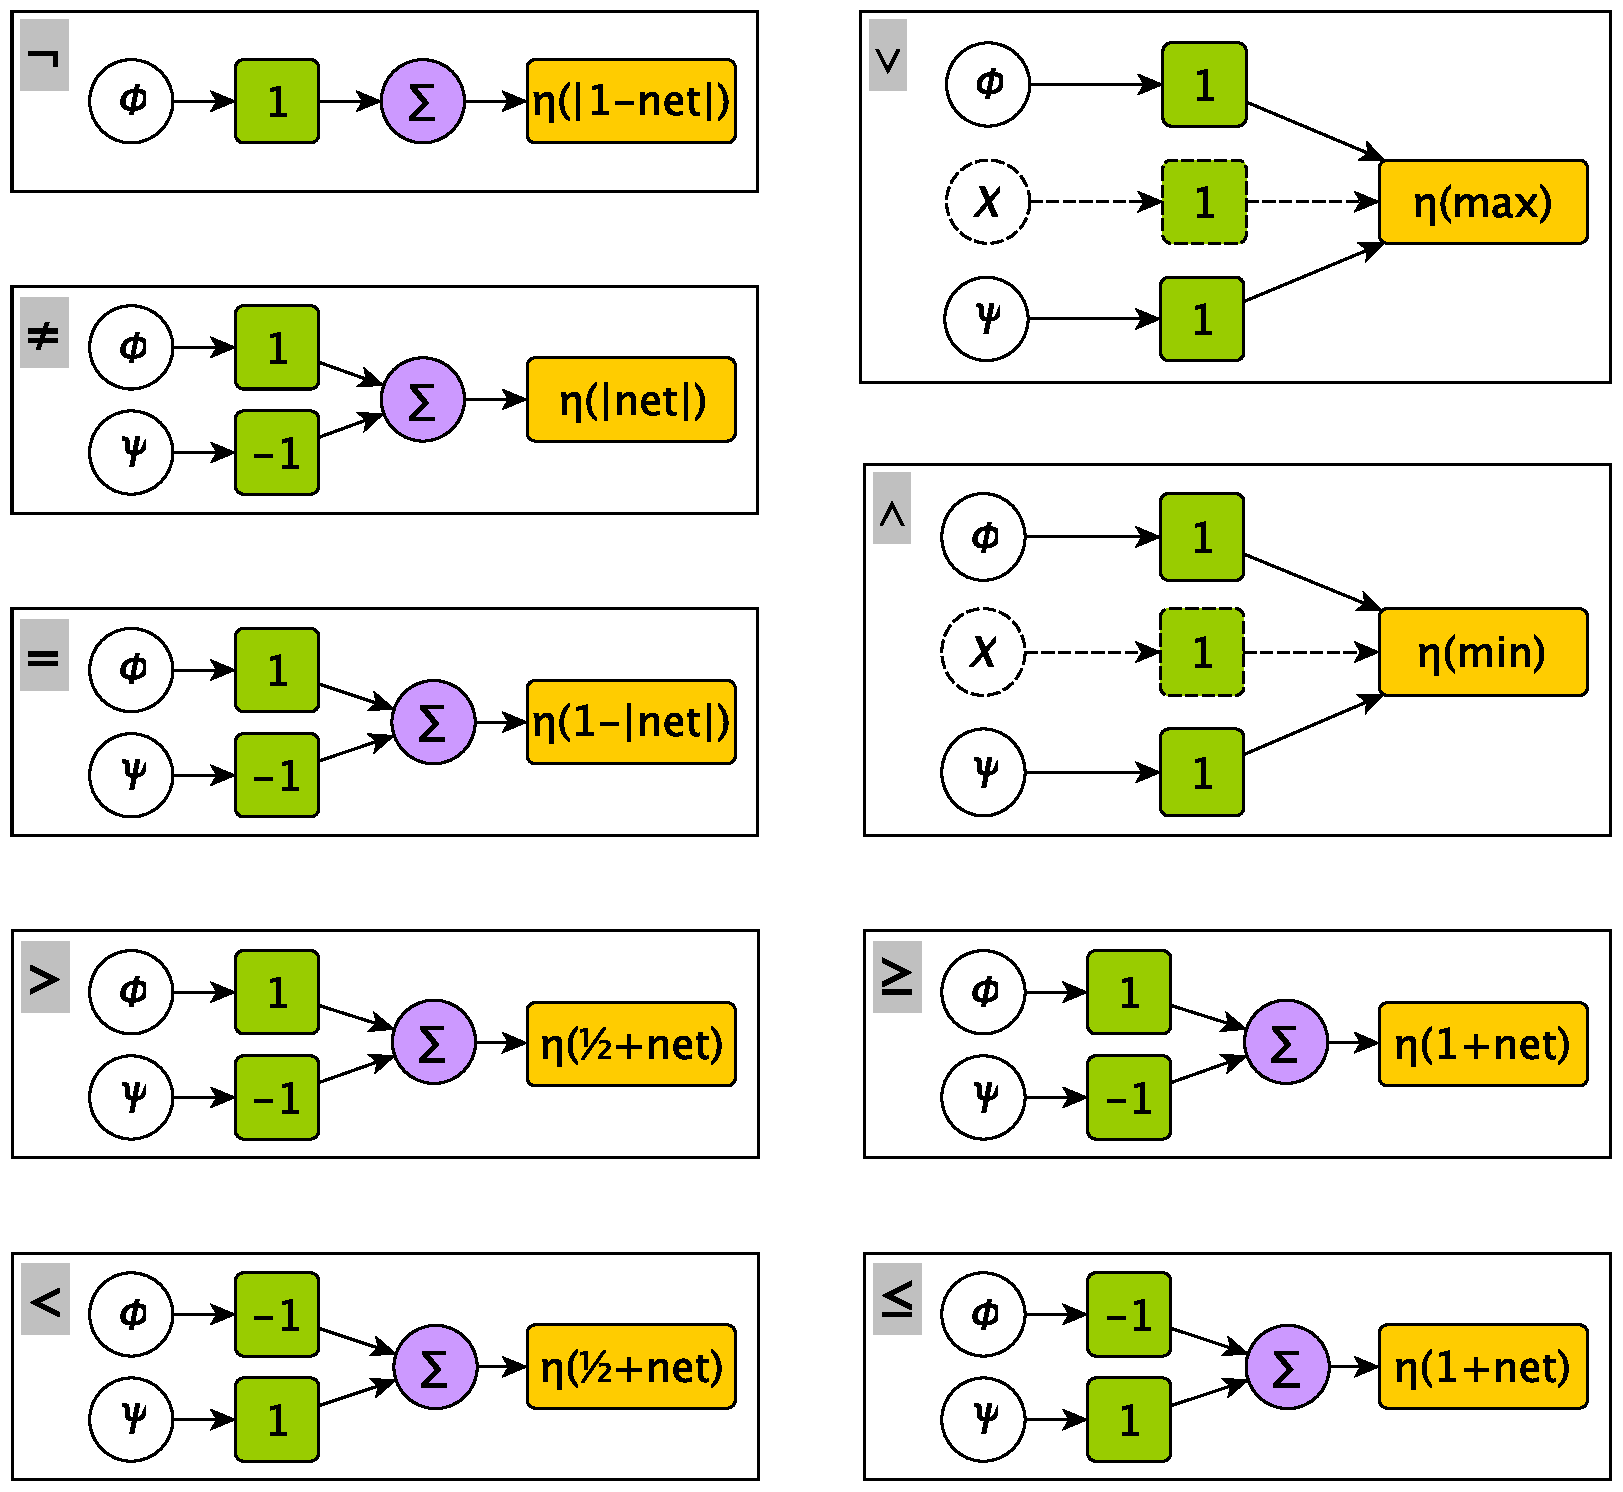
\includegraphics[width=0.65\textwidth]{figures/kins-fuzzifier-modules}
    \end{figure}
    
\end{frame}
%/////////

%/////////
\begin{frame}[allowframebreaks]{KILL: Knowledge Injection via Lambda Layer}
    TODO
\end{frame}
%/////////

%===============================================================================
\section{\psyki}
%===============================================================================

\begin{frame}[allowframebreaks]
\frametitle{Overall Design}

    \begin{center}
        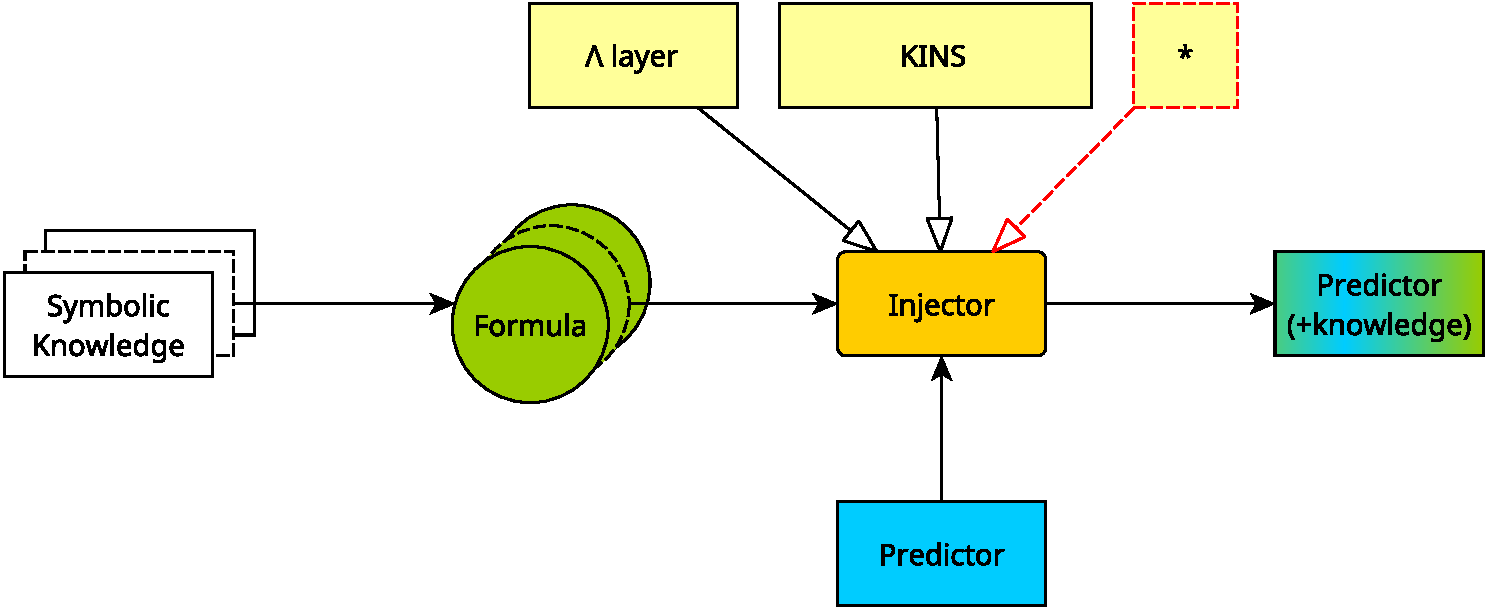
\includegraphics[width=\linewidth]{figures/psyki-design.pdf}
    \end{center}

    \framebreak

    Key components:
    %
    \begin{description}
        \item[injectior:] todo
        %
        \begin{itemize}
            \item details here
        \end{itemize}

        \item[predictor:] some trained classifier/regressor from which knowledge should be extracted
                
        \item[formula:] 
    \end{description}

    \begin{block}{Unified API for SKI}
        \begin{itemize}
            \item 1 interface for \kt{Injector}, several implementations
            %
            \begin{itemize}
                \item[eg] KILL, KINS, etc.
            \end{itemize}
            \item 1 interface for \kt{Formula}, several implementations
            %
            \begin{itemize}
                \item[eg] FOL, Datalog, etc.
            \end{itemize}
            \item 1 interface for \kt{Predictor}, several implementations
            %
            \begin{itemize}
                \item[eg] NN, kNN, DT
            \end{itemize}
        \end{itemize}
    \end{block}
\end{frame}

\begin{frame}[allowframebreaks]
\frametitle{API Design}

    \begin{center}
        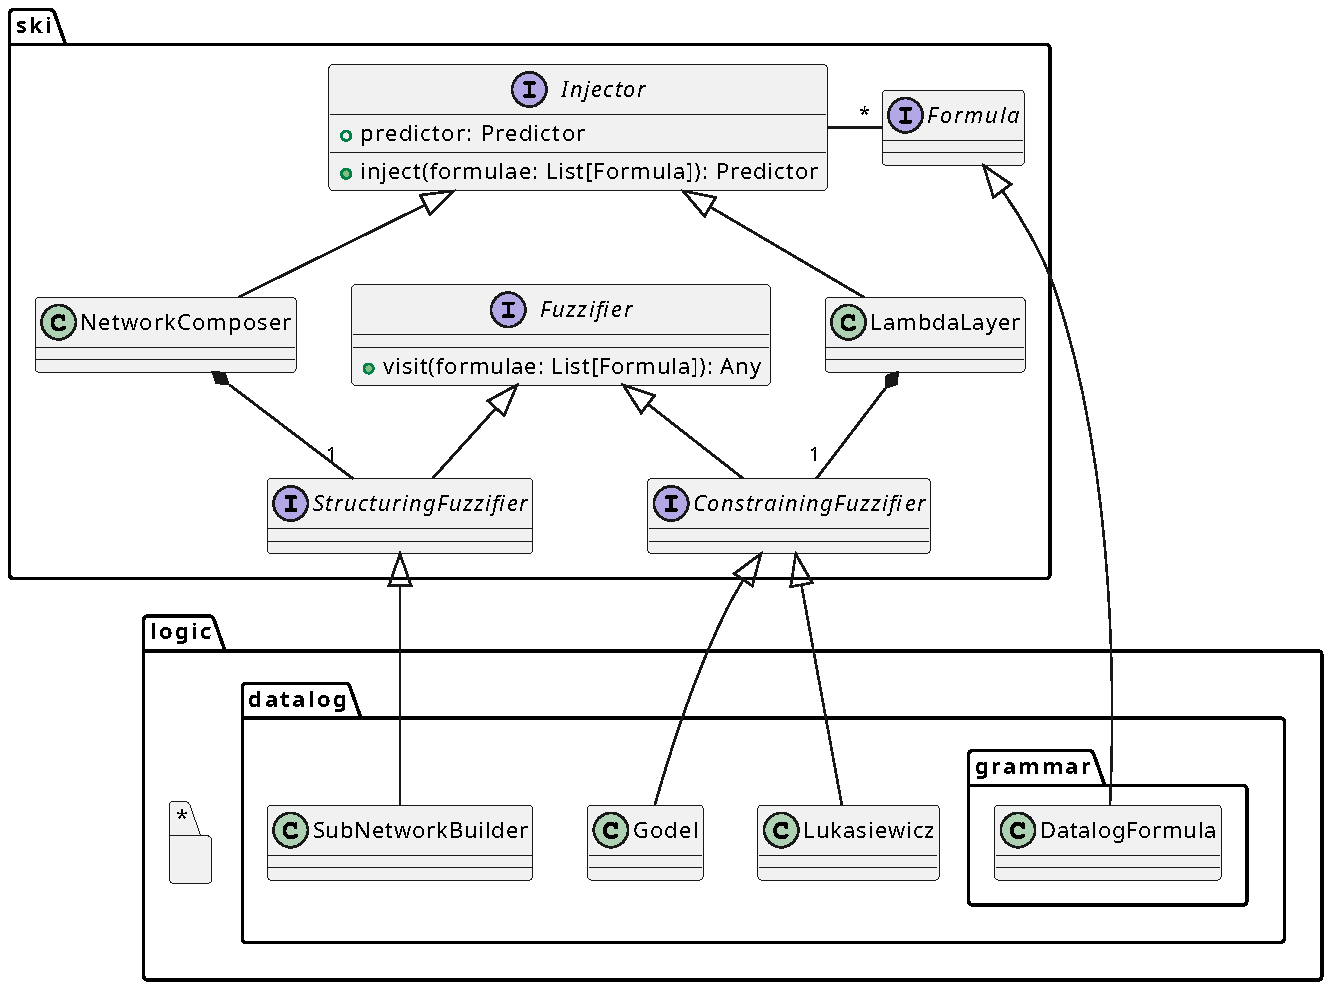
\includegraphics[width=.7\linewidth]{figures/psyki-class-diagram.pdf}
    \end{center}

    \framebreak

    Comments: TODO
\end{frame}


%===============================================================================
\section{Tutorial}
%===============================================================================

\begin{frame}{Tutorial}

    Two ways to reproduce the tutorial:
    
    \begin{block}{GitHub Repository (long way)}\centering
        \alert{\url{https://github.com/pikalab-unibo/prima-tutorial-2022}}
    \end{block}

    \begin{block}{DockerHub Images (quick way)}\centering
        \alert{\url{https://hub.docker.com/r/pikalab/prima-tutorial-2022/tags}}
    \end{block}
\end{frame}

\subsection{From GitHub}

\begin{frame}[allowframebreaks]{How to set the tutorial up from GitHub}

    \begin{block}{Enviromental pre-requisites}
        \begin{itemize}
            \item Python \alert{\texttt{3.9.x}}
            \item JDK \alert{$\geq$ \texttt{11}}
            \item Git
        \end{itemize}
    \end{block}

    \begin{enumerate}
        \item \texttt{git clone https://github.com/pikalab-unibo/prima-tutorial-2022}
        \item \texttt{cd prima-tutorial-2022}
        \item \texttt{pip install -r requirements.txt}
        \item \texttt{jupyter notebook}
        \framebreak
        \item Your browser should automatically open showing the following page:
        %
        \begin{center}
            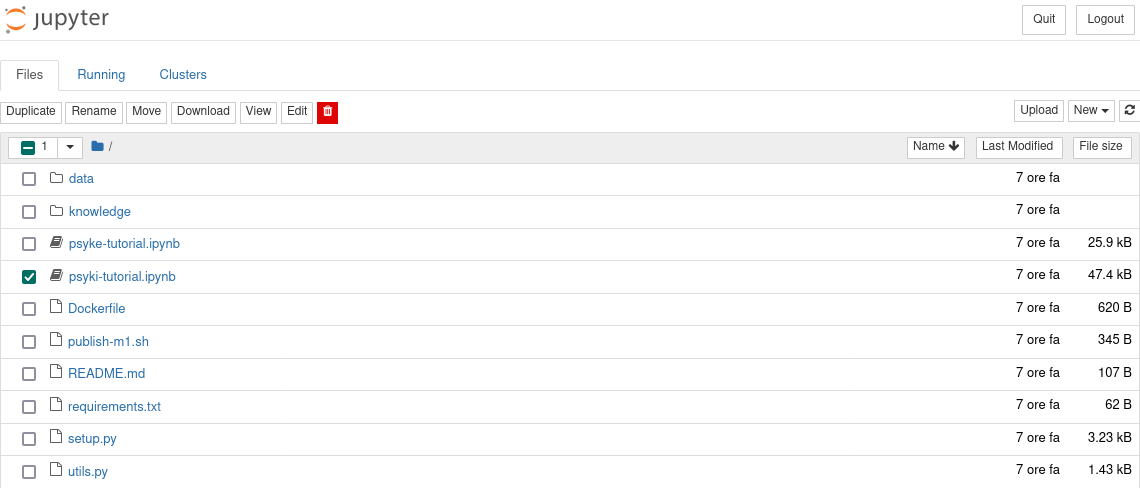
\includegraphics[width=.7\linewidth]{figures/jupyter-git.png}
        \end{center}
        \item open the \texttt{psyki-tutorial.ipynb} notebook
        \item listen to the speaker presenting the tutorial =)
    \end{enumerate}
\end{frame}

\subsection{From DockerHub}

\begin{frame}[allowframebreaks]{How to set the tutorial up via Docker}

    \begin{block}{Enviromental pre-requisites}
        \begin{itemize}
            \item Docker
        \end{itemize}
    \end{block}

    \begin{enumerate}
        \item \texttt{DOCKER\_IMAGE=}$\begin{cases}
            \texttt{pikalab/prima-tutorial-2022:latest} & \text{on most computers}
            \\
            \texttt{pikalab/prima-tutorial-2022:latest\alert{-apple-m1}} & \text{on Apple M1 computers}
        \end{cases}$
        \item \texttt{docker pull \$DOCKER\_IMAGE}
        %
        \begin{itemize}
            \item in case of lacking Internet access:
            %
            \begin{center}\ttfamily
                docker image load -i /path/to/local/image/file.tar
            \end{center}
        \end{itemize}
        \item \texttt{docker run -it --rm --name prima-tutorial-ske-ski -p 8888:8888 \$DOCKER\_IMAGE}
        \item Some textual output such as the following one should appear:
        %
        \lstinputlisting[basicstyle=\tiny\ttfamily]{listings/docker-logs.txt}
        \framebreak
        \item Copy-paste into your browser any link of the form: 
        %
        \begin{center}
            \alert{\texttt{http://cb0a3641caf0:8888/?token=\textit{TOKEN}}}
        \end{center}
        %
        \item Your browser should now be showing the following page:
        %
        \begin{center}
            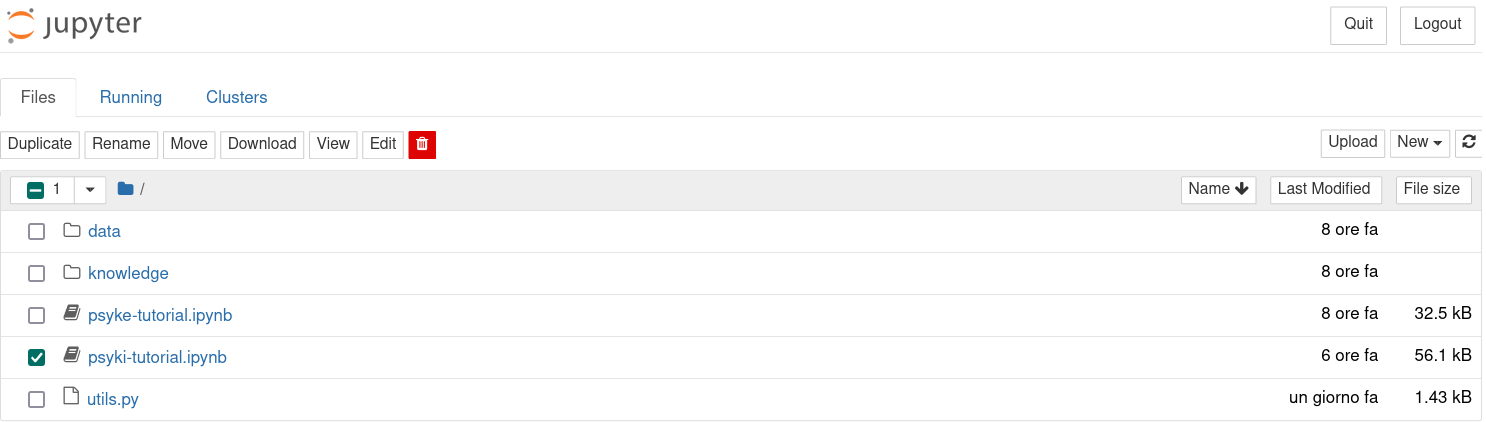
\includegraphics[width=.7\linewidth]{figures/jupyter-docker.png}
        \end{center}
        \item open the \texttt{psyki-tutorial.ipynb} notebook
        \item listen to the speaker presenting the tutorial =)
    \end{enumerate}
\end{frame}

%===============================================================================
\section{Discussion}
%===============================================================================

\begin{frame}{Notable Remarks}
    \begin{itemize}
        \item stuff
    \end{itemize}
\end{frame}

\begin{frame}{Current Limitations}
    \begin{itemize}
        \item todo
    \end{itemize}
\end{frame}

\begin{frame}{Future research activities}
    \begin{itemize}
        \item todo
    \end{itemize}
\end{frame}

%===============================================================================
\section*{}
%===============================================================================

%/////////
\frame{\titlepage}
%/////////

%===============================================================================
\section*{\refname}
%===============================================================================

%%%%
\setbeamertemplate{page number in head/foot}{}
%/////////
% \begin{frame}[c,noframenumbering]{\refname}
\begin{frame}[t,allowframebreaks,noframenumbering]{\refname}
%	\tiny
    \scriptsize
%	\footnotesize
    \bibliographystyle{apalike-AMS}
    \bibliography{psyki-tutorial}
\end{frame}
%/////////

%%%%%%%%%%%%%%%%%%%%%%%%%%%%%%%%%%%%%%%%%%%%%%%%%%%%%%%%%%%%%%%%%%%%%%%%%%%%%%%%
\end{document}
%%%%%%%%%%%%%%%%%%%%%%%%%%%%%%%%%%%%%%%%%%%%%%%%%%%%%%%%%%%%%%%%%%%%%%%%%%%%%%%%
